\documentclass{oci}
\usepackage[utf8]{inputenc}
\usepackage{lipsum}
\usepackage{tikz}

\title{Ejemplo}

\begin{document}
\begin{problemDescription}
  Hace algunas semanas Gastón por fin cumplió el sueño de la casa propia.
  Lamentablemente, antes de poder mudarse hay muchas cosas que debe arreglar.
  La que más le urge es renovar la cocina.
  Para poder renovarla lo primero que debe hacer es cambiar por completo las
  baldosas.

  La cocina en la nueva casa de Gastón es de $M$ centímetros de largo y $N$
  centímetros de ancho.
  Las baldosas que desea comprar son de $a$ centímetros de largo y $b$ de ancho.
  Para poder embaldosar la cocina Gastón debe partir poniendo una baldosa en una
  de las esquinas y continuar poniendo baldosas una al lado de la otra hasta
  completar una fila.
  Si la última baldosa en la fila no cabe completamente puede cortarla para
  poder llenar el espacio faltante.
  Luego de completar una fila puede seguir con la siguiente.
  Al llegar a la última fila, si las baldosa no caben completamente, puede
  también cortar las baldosas que pondrá en esa fila.
  Gastón está interesado en saber cuantas baldosas necesitará para poder cubrir
  completamente el piso de la cocina.

  La siguiente figura muestra un ejemplo con una cocina de 14 por 7 centímetros,
  y baldosas de 3 por 2 centímetros.
  Como puede apreciarse, en este caso es necesario un total de 20 baldosas para
  poder cubrir todo el piso.
  \begin{center}
    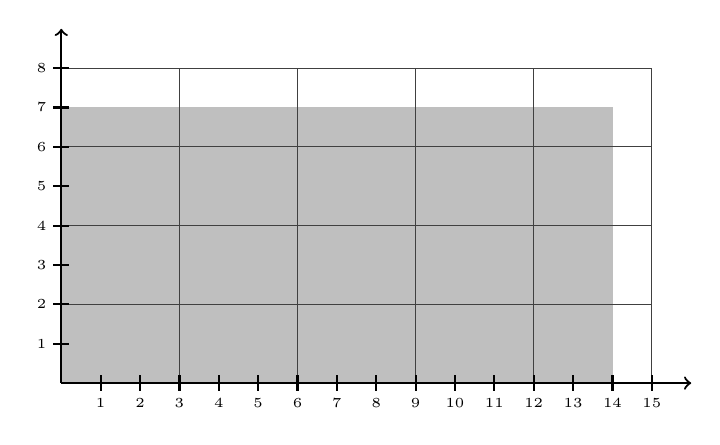
\begin{tikzpicture}[scale=0.5]
      \draw [lightgray, fill=lightgray] (0, 0) rectangle (14, 7);
      \foreach \i in {0,...,4}{
          \foreach \j in {0,...,3}{
            \draw [darkgray] (3*\i, 2*\j) rectangle +(3,2);
          }
        }
      \draw [thick, ->] (0, 0) -- (0, 9);
      \foreach \i in {1,...,8} {
        \draw [thick] (-0.2, \i) -- (0.2, \i);
        \node at (-0.5, \i) {\tiny\i};
      }
      \draw [thick, ->] (0, 0) -- (16, 0);
      \foreach \i in {1,...,15} {
        \draw [thick] (\i, -0.2) -- (\i, 0.2);
        \node at (\i, -0.5) {\tiny\i};
      }
    \end{tikzpicture}
  \end{center}
\end{problemDescription}

\begin{inputDescription}
  La primera línea de la entrada contiene dos enteros $M$ y $N$ ($0 < M, N \leq
  10000$), correspondientes respectivamente al largo y ancho de la cocina en
  centímetros.
  La siguiente línea contiene dos enteros $a$ y $b$ ($0 < M, N \leq 100$)
  correspondiente al largo y ancho de la baldosa en centímetros.
\end{inputDescription}

\begin{outputDescription}
  La salida debe contener un único entero correspondiente a la cantidad de
  baldosas necesarias para poder cubrir completamente el piso de la cocina.
\end{outputDescription}

\section*{Subtareas y puntaje}
Este problema no contiene subtareas.
Se dará una cantidad de puntos proporcional a la cantidad de casos de prueba
correctos.
\begin{sampleDescription}
\sampleIO{sample-1}
\sampleIO{sample-2}
\end{sampleDescription}

\end{document}
